% Author: Marek Fiser <tikz at marekfiser.cz>
% MESIF protocol: http://en.wikipedia.org/wiki/MESIF_protocol
\documentclass[tikz, border=10pt]{standalone}
%%%<
\usepackage{verbatim}
\usetikzlibrary{calc}
\usetikzlibrary{fit}
%%%>
\begin{comment}
:Title: MESIF protocol
:Tags: Diagrams;Block diagrams;Computer science
:Author: Marek Fiser
:Slug: mesif

A diagram describing the MESIF protocol: http://en.wikipedia.org/wiki/MESIF_protocol
\end{comment}
\usetikzlibrary{arrows}
\begin{document}
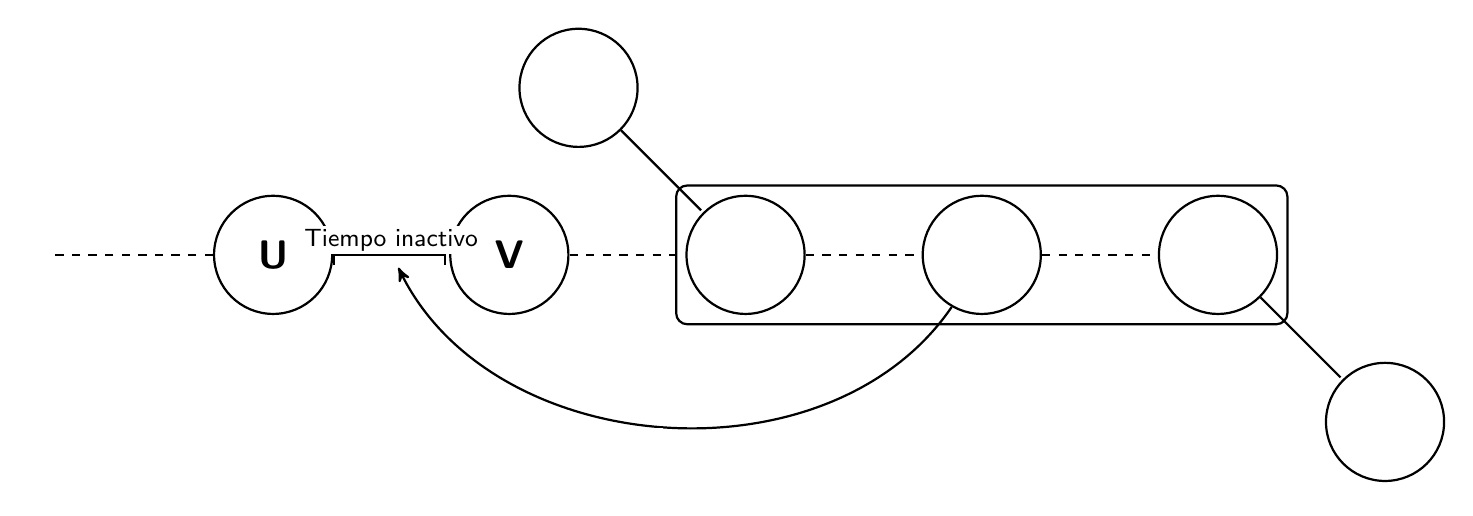
\begin{tikzpicture}[->,>=stealth',shorten >=1pt,auto,node distance=3cm,
  thick,main node/.style={circle,fill=white!20,draw,
  font=\sffamily\Large\bfseries,minimum size=15mm}]
  \node[main node] (M) {U};
  \node (JPM)[left of=M] {};
  \node[main node] (E) [right of=M] {V};
  \node (aux) at ($(M)!0.5!(E)$) {};
  %\node (lab) at ($(aux)$) {Tiempo inactivo en la máquina};
  \node[main node] (S) [right of=E] {};
  \node[main node] (JPS) [above left of=S]{};
  \node[main node] (F) [right of=S] {};
  \node[main node] (I) [right of=F] {};
  \node[main node] (JSI) [below right of=I] {};

  \draw[|-|] (M)--(E);

  \path[every node/.style={font=\sffamily\small,
  		fill=white,inner sep=1pt}]
  	% Right-hand-side arrows rendered from top to bottom to
  	% aristas
    (M) edge [|-|] node {Tiempo inactivo} (E)
  	(M) edge[dashed,-] node {} (JPM)
    (E) edge [dashed,-] node {} (S)
  	(JPS) edge[-] node {} (S)
    (S) edge [dashed,-] node {} (F)
    (F) edge [dashed,-] node {} (I)
    (I) edge [-] node{} (JSI)
    % flechas de movimimiento 
    (F) edge [bend left=60] node{} (aux);
    (lab) edge node{labl} (aux);
    %(E) edge [bend left=30] node {} (S)
    %(S) edge [bend left=30] node{} (F)
    %(F) edge [bend left=30] node {} (I);
     \node[draw,rounded corners,fit= (S) (F) (I)] {};
  	% Left-hand-side arrows rendered from bottom to top to
  	% achieve proper rendering of labels over arrows.
%    (I) edge [bend left=65] node[left=1mm] {PrWr/BusRdX} (M)
%        edge [bend left=55] node[left=1mm] {PrRd/BusRd Ex} (E)
%        edge [bend left=30] node[left=1mm] {PrRd/BusRd} (F)
%    (F) edge [loop above] node {PrRd/-} (F)
%        edge [bend left=50] node[left=1mm] {PrWr/BusRdX} (M)
%        edge [bend left=30] node[left=1mm] {BusRd/Flush} (S)
%    (S) edge [bend left=40] node[left=1mm] {PrWr/BusRdX} (M)
%    (E) edge [bend left=30] node[left=1mm] {PrWr/-} (M);
\end{tikzpicture}
\end{document}
